\documentclass[rpussian]{beamer}

\usepackage{cmap} % для кодировки шрифтов в pdf
\usepackage[T2A]{fontenc}
\usepackage[utf8]{inputenc}
\usepackage[russian]{babel}
\usepackage{minted} % code highlighting

\usepackage{graphicx} % для вставки картинок
\graphicspath{ {img/} }

%\usetheme{Rochester}
\usecolortheme{wolverine}
\definecolor{bg}{rgb}{0.95,0.95,0.95}


\title{Неизменяемые структуры данных в Clojure}
\author{Белоглазов Никита}
\date{2013}
\institute{Белорусский Государственный Университет}

\begin{document}

\maketitle
\begin{frame}[fragile]
  \begin{description} \itemsep1cm
  \item вектор (vector)
    \begin{itemize}
    \item ArrayList, java
    \item PersistentVector, clojure
    \end{itemize}
  \item отображение (map)
    \begin{itemize}
    \item HashMap, java
    \item PersistentHashMap, clojure
    \end{itemize}
  \end{description}
\end{frame}

\begin{frame}[fragile]
  \frametitle{ArrayList}
  \begin{itemize}
  \item внутри содержит массив фиксированного размера
  \item при заполнении массива все элементы копируются в новый массив бoльшего размера
  \end{itemize}
  \begin{minted}[bgcolor=bg,gobble=4,frame=single]{java}
    public class ArrayList<E> {

        private transient Object[] elementData;

        private int size;

        // constructors, methods
    }
  \end{minted}
\end{frame}

\begin{frame}
  \frametitle{PersistentVector: представленив}
  Вектор является 32-ричным деревом \\
  \vspace{1cm}
  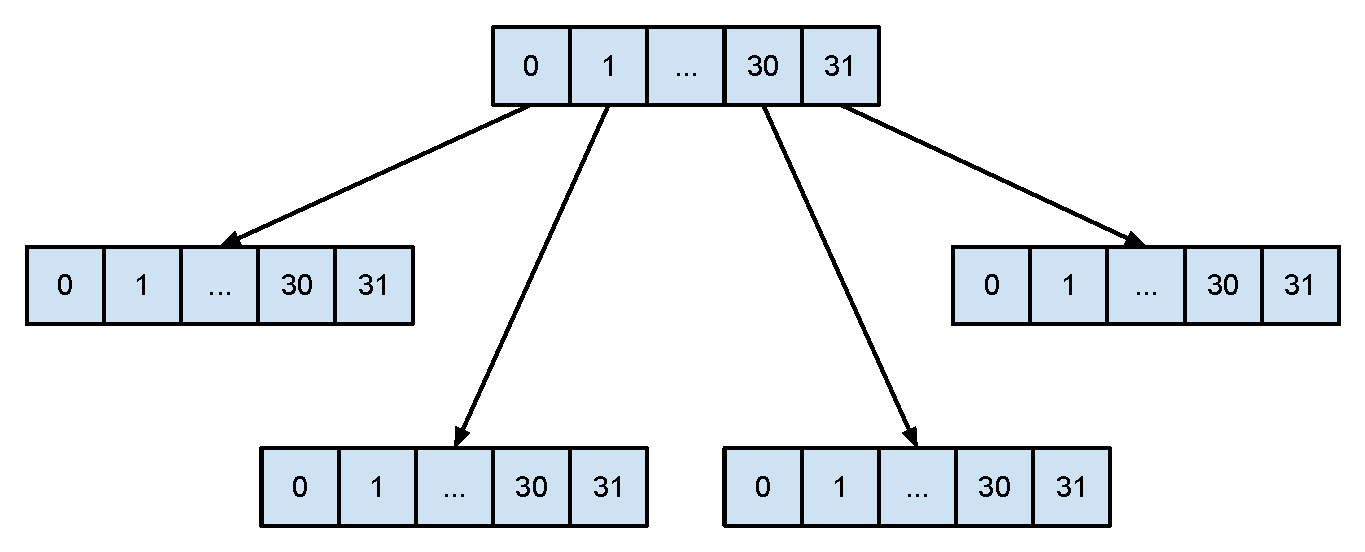
\includegraphics[width=\textwidth,keepaspectration]{32tree}
\end{frame}

\begin{frame}
  \frametitle{PersistentVector: индексы}
  \begin{itemize}
  \item битовая запись индекса разбивается на группы по 5 бит
  \item каждая группа кодирует число (0-31) - номер ячейки на определённом уровне дерева
  \end{itemize}
  \\ \vspace{0.5cm}
  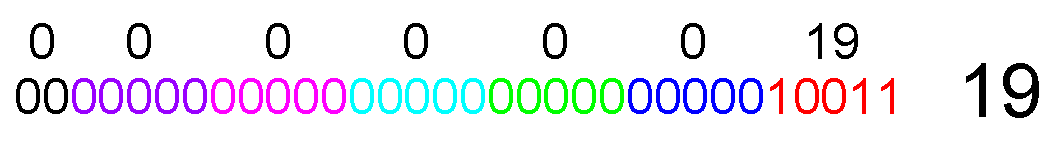
\includegraphics[width=\textwidth,keepaspectration]{bits_19}
  \\ \vspace{0.5cm}
  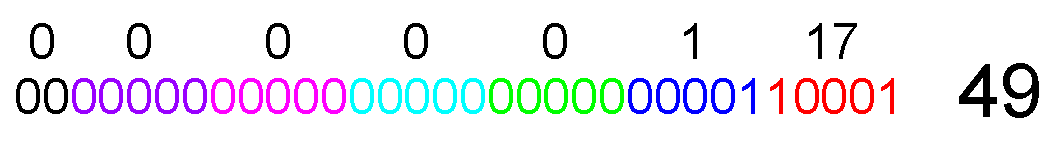
\includegraphics[width=\textwidth,keepaspectration]{bits_49}
\end{frame}

\begin{frame}
  \frametitle{PersistentVector: добавление элементов}
  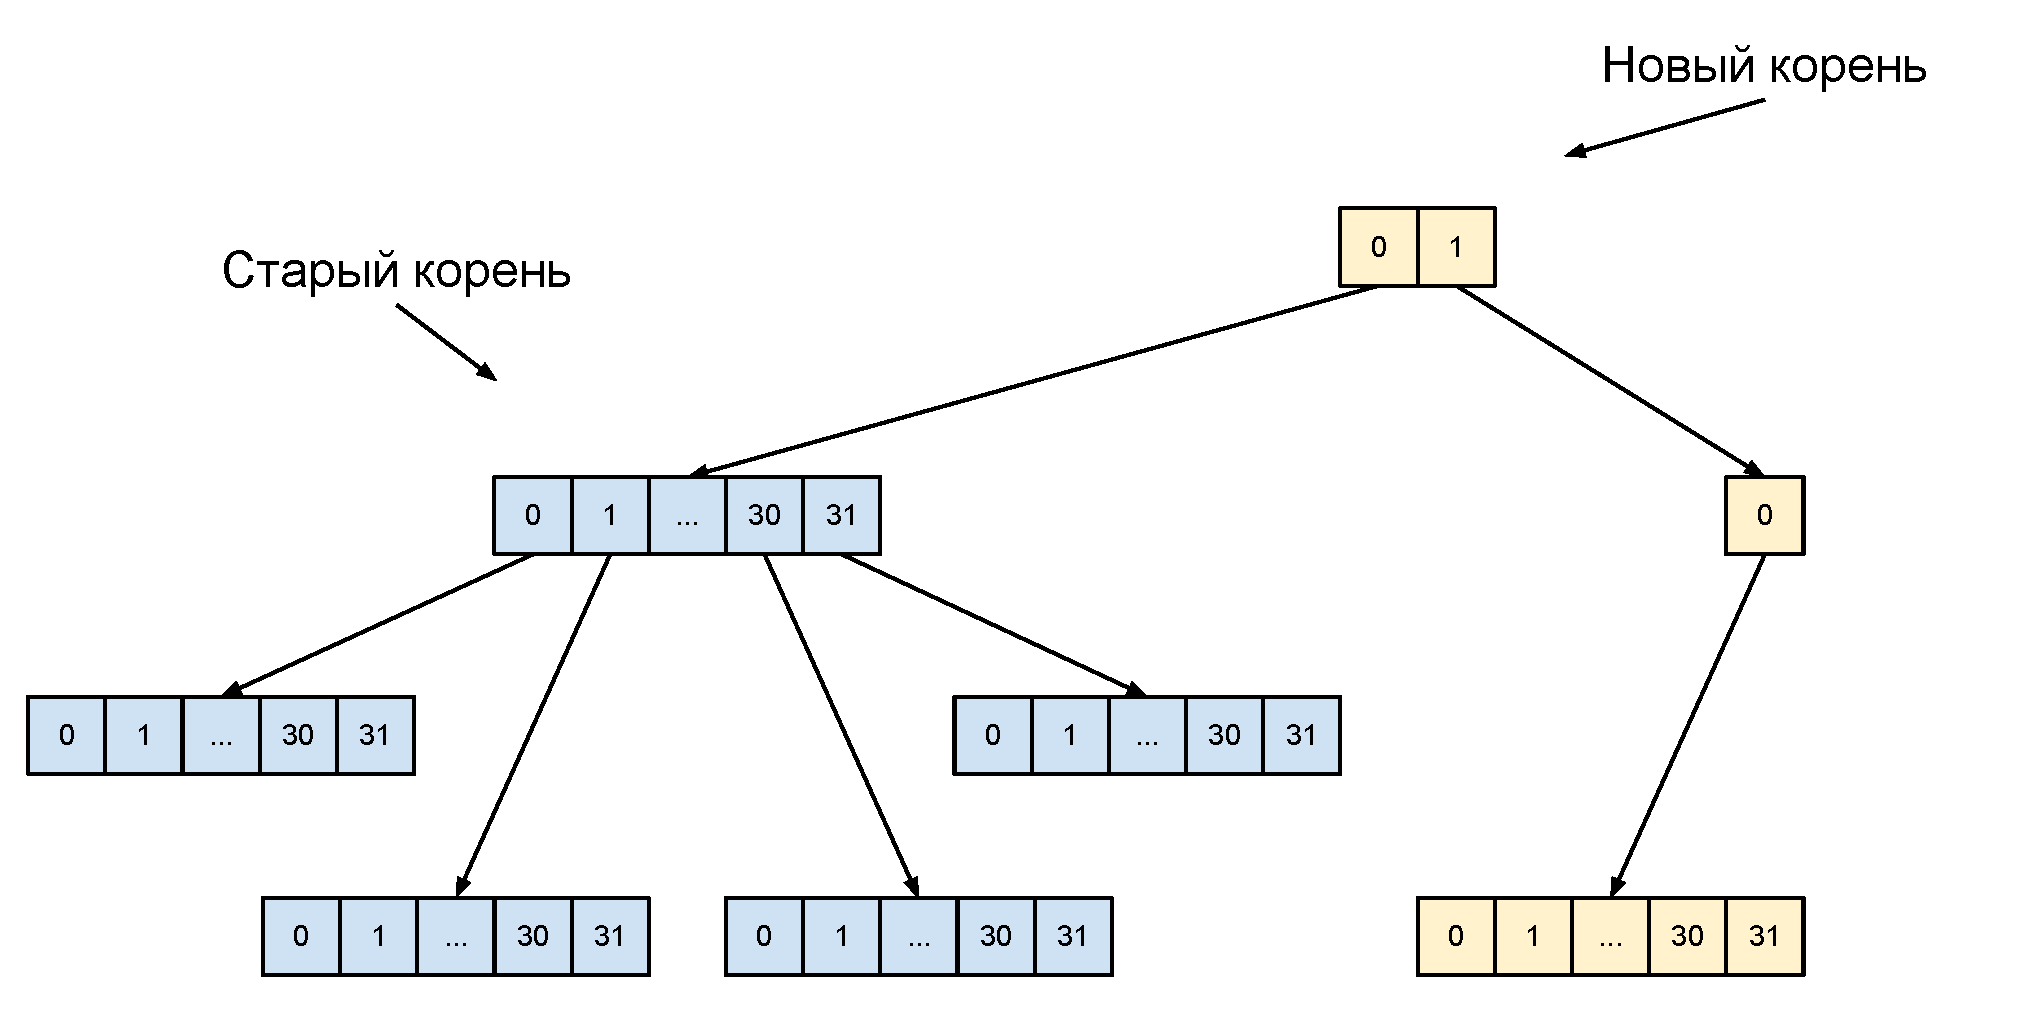
\includegraphics[width=\textwidth,keepaspectration]{32_tree_added_1}
\end{frame}

\begin{frame}[fragile]
  \frametitle{PersistentVector: состав}
  \begin{minted}[bgcolor=bg,gobble=4,linenos=true]{java}
    public class PersistentVector {

      public static class Node {
        public final AtomicReference<Thread> edit;
        public final Object[] array;
      }

      final int cnt;
      public final int shift;
      public final Node root;
      public final Object[] tail;
      final IPersistentMap _meta;

      // constructors, methods
    }
  \end{minted}
\end{frame}

\begin{frame}[fragile]
  \frametitle{PersistentVector: nth}
  \begin{minted}[bgcolor=bg,gobble=4,linenos=true]{java}
    public Object nth(int i) {
      Object[] node = arrayFor(i);
      return node[i & 0x01f];
    }

    public Object[] arrayFor(int i) {
      if(i >= 0 && i < cnt) {
        if(i >= tailoff())
          return tail;
        Node node = root;
        for(int level = shift; level > 0; level -= 5)
          node = (Node) node.array[(i >>> level) & 0x01f];
        return node.array;
      }
      throw new IndexOutOfBoundsException();
    }

  \end{minted}
\end{frame}

\begin{frame}
  \frametitle{HashMap: структура}
  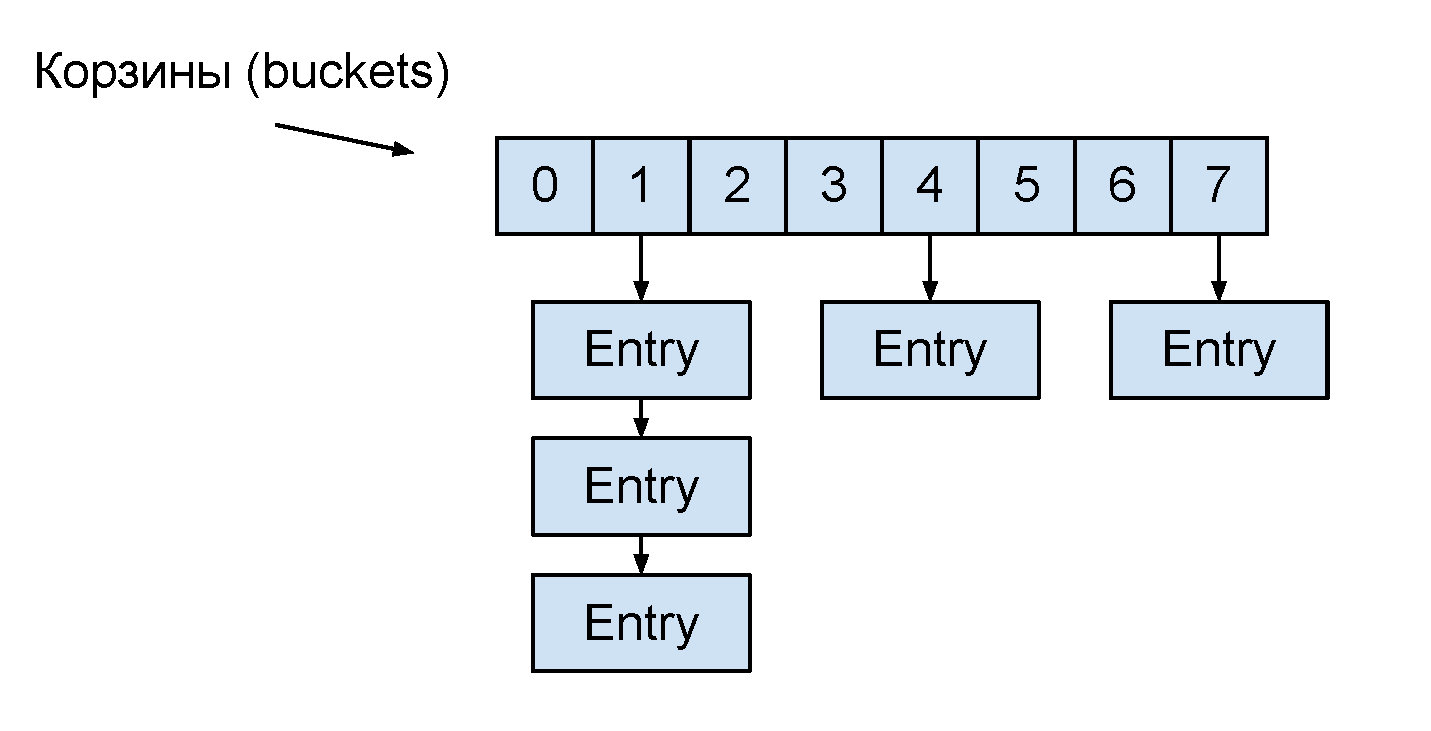
\includegraphics[width=\textwidth,keepaspectration]{hashmap}
\end{frame}

\begin{frame}[fragile]
  \frametitle{HashMap: состав}
  \begin{minted}[bgcolor=bg,gobble=4,linenos=true]{java}
    public class HashMap<K,V> {

      transient Entry[] table;
      transient int size;
      int threshold;
      final float loadFactor;
      transient volatile int modCount;

      static class Entry<K,V> {
        final K key;
        V value;
        Entry<K,V> next;
        final int hash;
      }

      // constructors, methods
    }
  \end{minted}
\end{frame}

\begin{frame}
  \frametitle{Конец}
  \begin{columns}[c]
    \begin{column}{.5\textwidth}
      \begin{center}
        Спасибо за внимание!
        \\ \vspace{1cm}
        Вопросы?
      \end{center}
    \end{column}
    \begin{column}{.5\textwidth}
      
\includegraphics[width=\textwidth,keepaspectration]{alien}
    \end{column}
  \end{columns}
\end{frame}

\end{document}

%%% Local Variables:
%%% mode: latex
%%% TeX-master: t
%%% End:
